
% This LaTeX was auto-generated from MATLAB code.
% To make changes, update the MATLAB code and republish this document.

\documentclass{article}
\usepackage{graphicx}
\usepackage{color}

\sloppy
\definecolor{lightgray}{gray}{0.5}
\setlength{\parindent}{0pt}

\begin{document}

    
    
\section*{Zachary Kaplan}

\begin{par}
Math 440 Computational Lab \#4 5/3/19
\end{par} \vspace{1em}

\subsection*{Contents}

\begin{itemize}
\setlength{\itemsep}{-1ex}
   \item An Elliptic PDE Instance
   \item C.5.1.1 - Numerically Solve the PDE
   \item Derivation of the Analytic Solution.
   \item Why is the numerical result exact?
   \item Comparison to results from LU factorization solver.
   \item Helper Functions
\end{itemize}
\begin{par}
An online version of this file can be found published to: https://www.overleaf.com/read/wwdtnstrvpqz
\end{par} \vspace{1em}
\begin{par}
\textbf{NOTE}: To render this file locally, please prepend the following package         dependencies to the latex generated by matlab publish:
\end{par} \vspace{1em}

\begin{verbatim}\usepackage[margin=1in]{geometry}
\usepackage{amsmath}
\usepackage{amssymb}
\usepackage{microtype}
\usepackage{csquotes}
\usepackage{bm}\end{verbatim}
    \begin{par}
It is also recommended to use the following command to stop matrices from wrapping.
\end{par} \vspace{1em}

\begin{verbatim}\setcounter{MaxMatrixCols}{20}\end{verbatim}
    

\subsection*{An Elliptic PDE Instance}

\begin{par}
Consider a 2D metal block denoted by the region $\Omega = [0,4] \times [0, 2]$. The following PDE defines the temperature distribution throughout the block given von Neumann Boundary Conditions on the upper and lower boundaries, and Dirichlet Boundary Conditions on the left and right boundaries.
\end{par} \vspace{1em}
\begin{par}
$$ \begin{aligned}
 \nabla^2 T = 0, && \forall~(x,y) \in \Omega \\
 T(0, y) = 300, && T(4, y) = 600, && \forall~y \in [0, 2] \\
 \frac{\partial T}{\partial y}(x, 0) = 0,
   && \frac{\partial T}{\partial y}(x, 2) = 0,
   && \forall~x \in [0, 4] \\
\end{aligned} $$
\end{par} \vspace{1em}


\subsection*{C.5.1.1 - Numerically Solve the PDE}

\begin{par}
First, we discretize space using a uniform stepsize $h$ as suggested in the text, with ghost points along $y = -h$ and $y = 2+h$. This results in a grid of points $x_{ij}$ where $x_{ij} = (x_j, y_i) = (hj, h(i-1)),  \forall~ i = 0, 1, \ldots, M+1 = 2/h + 2~\text{and}~  j = 0, 1, \ldots, N+1 = 4/h$. We then define our approximate solution $T_{ij} = T(x_{ij}) = T(x_j, y_i)$.
\end{par} \vspace{1em}
\begin{par}
Now we define our FD approximations for the derivatives in our PDE system:
\end{par} \vspace{1em}
\begin{par}
$$ \begin{aligned}
 \nabla^2T(x_j, y_i) &\approx
   \frac{T_{i+1,j} - 2T_{ij} + T_{i-1,j}}{h^2} +
   \frac{T_{i,j+1} - 2T_{ij} + T_{i,j-1}}{h^2} \\
   &= \frac{1}{h^2}
   \left( T_{i+1,j} + T_{i-1,j} + T_{i,j+1} + T_{i,j-1} - 4T_{ij}\right)
   = 0 && \forall~i = 1, 2, \ldots, M~\text{and}~j= 1, 2, \ldots, N  \\
 \frac{\partial T}{\partial y}(x_j, 0)
   &\approx \frac{T_{2j} - T_{0j}}{2h} = 0
    && \forall~j = 1, 2, \ldots, N \\
 \frac{\partial T}{\partial y}(x_j, 2)
   &\approx \frac{T_{M+1,j} - T_{M-1,j}}{2h} = 0
    && \forall~j = 1, 2, \ldots, N \\
 T(0, y_i) &\approx T_{i0} = 300, \quad T(4, y_i) \approx T_{i,N+1} = 600
   && \forall~i = 1, 2, \ldots, M
\end{aligned} $$
\end{par} \vspace{1em}
\begin{par}
Notice that none of the above constraints operate on the values $T_{00}, T_{0,N+1}, T_{M+1,0}, T_{M+1,N+1}$. Since none of these values are in $\overline{\Omega}$, we just set them explicitly to 0.
\end{par} \vspace{1em}
\begin{par}
Let the vector $\bm{T} = \begin{pmatrix} T_{00}, T_{10}, \ldots,                           T_{M+1,0}, T_{01}, T_{11}, \ldots,                           T_{M,N+1}, T_{M+1,N+1} \end{pmatrix}^\top$ be a flattened representation of our approximate solution $T_{ij}$. Then we can represent the PDE constraints of our system as
\end{par} \vspace{1em}
\begin{par}
$$ \begin{aligned}
 A_1 \bm{T} &= \bm0_{NM}^\top, \\
 A_1 &= \begin{pmatrix}
  0 &  1 & 0 & \bm{0}_{M-1} &
  1 & -4 & 1 & \bm{0}_{M-1} &
  0 &  1 & 0 & \multicolumn{5}{c}{\cdots} & 0 \\
  0 & 0 &  1 & 0 & \bm{0}_{M-1} &
      1 & -4 & 1 & \bm{0}_{M-1} &
      0 &  1 & 0 & \multicolumn{4}{c}{\cdots} & 0 \\
  0 & 0 &      0 & \ddots & \ddots & \ddots
        & \ddots & \ddots & \ddots & \ddots
        & \ddots & \ddots & 0 & \multicolumn{3}{c}{\cdots} & 0 \\
  \multicolumn{17}{c}{\vdots} \\
  \bm{0}_{M-1} & 0 &  1 & 0 & \bm{0}_{M-1} &
                 1 & -4 & 1 & \bm{0}_{M-1} &
                 0 &  1 & 0 & \multicolumn{4}{c}{\cdots} & 0 \\
  \bm{0}_{M-1} & 0 & 0 & 0 & 0 &  1 & 0 & \bm{0}_{M-1} &
                             1 & -4 & 1 & \bm{0}_{M-1} &
                             0 &  1 & 0 & \cdots & 0 \\
  \multicolumn{17}{c}{\vdots} \\
  0 & \multicolumn{4}{c}{\cdots} & 0 &  1 & 0 & \bm{0}_{M-1} &
                                   1 & -4 & 0 & \bm{0}_{M-1} &
                                   0 &  1 & 0 & 0 \\
  0 & \multicolumn{4}{c}{\cdots} & 0 & 0 &  1 & 0 & \bm{0}_{M-1} &
                                   1 & -4 & 0 & \bm{0}_{M-1} &
                                   0 &  1 & 0 \\
 \end{pmatrix}.
\end{aligned} $$
\end{par} \vspace{1em}
\begin{par}
Notice that $A_1 \in \mathbb{R}^{NM \times (N+2)(M+2)}$ and is made up of $N$ banded blocks of $M$ equations each. Each block shares the same band $\begin{pmatrix} 0 &  1 & 0 & \bm{0}_{M-1} &                       1 & -4 & 0 & \bm{0}_{M-1} &                       0 &  1 & 0 \end{pmatrix}$, and between each block there is an offset of 3 entries (as illustrated in the middle section of $A_1$ which shows the  border of block 1 and block 2). Another way to view this matrix is as a banded matrix with the above band justified at the top left corner where any row $k$ s.t. $k \equiv M+1~(\mod M+2)$ or $k \equiv M+2~(\mod M+2)$ is omitted.
\end{par} \vspace{1em}
\begin{par}
The von Neumann BCs can similarly be represented by a matrix system:
\end{par} \vspace{1em}
\begin{par}
$$ \begin{aligned}
 A_2 \bm{T} &= \bm{0}_{2N}^\top \\
 A_2 &= \begin{pmatrix}
  \bm{0}_{M+2}            & -1 & 0 & 1 & 0 & \cdots & 0 \\
  \bm{0}_{2(M+2) - 3}     & -1 & 0 & 1 & 0 & \cdots & 0 \\
  \bm{0}_{2(M+2)}         & -1 & 0 & 1 & 0 & \cdots & 0 \\
  \multicolumn{7}{c}{\vdots} \\
  \bm{0}_{N(M+2)}         & -1 & 0 & 1 & 0 & \cdots & 0 \\
  \bm{0}_{(N+1)(M+2) - 3} & -1 & 0 & 1 & \multicolumn{3}{c}{\bm{0}_{M+2}}
 \end{pmatrix}.
\end{aligned} $$
\end{par} \vspace{1em}
\begin{par}
Note that $A_2 \in \mathbb{R}^{2N \times (N+2)(M+2)}$ and is essentially a matrix with band $\begin{pmatrix} -1 & 0 & 1 \end{pmatrix}$ justified at the top left corner where only rows $k$ s.t. $k \equiv 1~(\mod M+2)$ or $k \equiv M~(\mod M+2)$ are included. Furthermore, rows $k = 1, M, (N+1)(M+2) + 1, (N+2)(M+2) - 2$ are omitted despite satisfying the modulus equations above (they would correspond to the BCs at $x_0$ and $x_{N+1}$).
\end{par} \vspace{1em}
\begin{par}
Finally, we can write our Dirichlet BCs and the constraints on the corners of our discrete grid as a simple matrix system:
\end{par} \vspace{1em}
\begin{par}
$$ \begin{aligned}
 A_3 \bm{T} &= \bm{b} \\
 A_3 &= \begin{pmatrix}
  0 & 1 & 0 & 0 & 0 & \cdots & 0 \\
  0 & 0 & 1 & 0 & 0 & \cdots & 0 \\
  0 & 0 & 0 & \ddots & 0 & \cdots & 0 \\
  \multicolumn{7}{c}{\vdots} \\
  \bm{0}_M & 1 & 0 & 0 & 0 & \cdots & 0 \\
  0 & \cdots & 0 & 0 & 1 & \multicolumn{2}{r}{\bm{0}_M} \\
  0 & \cdots & 0 & 0 & 0 & \ddots & \vdots \\
  \multicolumn{7}{c}{\vdots} \\
  0 & \cdots & 0 & 0 & 0 & 1 & 0 \\
  1 & 0 & 0 & 0 & 0 & \cdots & 0 \\
  \bm0_{M+1} & 1 & 0 & 0 & 0 & \cdots & 0 \\
  0 & \cdots & 0 & 0 & 0 & 1 & \bm0_{M+1} \\
  0 & \cdots & 0 & 0 & 0 & 0 & 1 \\
 \end{pmatrix},\quad
 \bm{b} = \begin{pmatrix}
   300 \cdot \bm{1}_{M}^\top \\ 600 \cdot \bm{1}_{M}^\top \\
   0 \\ 0 \\ 0 \\ 0
 \end{pmatrix}
\end{aligned} $$
\end{par} \vspace{1em}
\begin{par}
Notice that $A \in \mathbb{R}^{2M + 4 \times (M+2)(N+2)}$, and is essentially two identity matrix blocks, and the 4 corner constraints. Finally, we can represent all constraints in the matrix system given by
\end{par} \vspace{1em}
\begin{par}
$$
 \begin{pmatrix} A_1 \\ A_2 \\ A_3 \end{pmatrix} \bm T
   = \begin{pmatrix}
     \bm0_{NM} & \bm0_{2N} & 300 \cdot \bm1_N & 600 \cdot \bm1_N & \bm0_4
     \end{pmatrix}^\top.
$$
\end{par} \vspace{1em}
\begin{verbatim}
% Solve for both stepsizes.
h1 = 0.1;
h2 = 0.2;
[X1, Y1, T1, t1_backslash] = lab4_solve_backslash(h1);
[X2, Y2, T2, t2_backslash] = lab4_solve_backslash(h2);

% Plot both figures.
figure;
imagesc(X1, Y1, T1)
colorbar
xlabel('X');
ylabel('Y');
title(sprintf('Plot for solution with h = %.1f', h1));

figure;
imagesc(X2, Y2, T2)
colorbar
xlabel('X');
ylabel('Y');
title(sprintf('Plot for solution with h = %.1f', h2));

% Print the values at (1, 2).
fprintf('h = %.1f, T(1, 2) = %f\n', h1, full(T1(Y1 == 2, X1 == 1)));
fprintf('h = %.1f, T(1, 2) = %f\n', h2, full(T2(Y2 == 2, X2 == 1)));
\end{verbatim}


\subsection*{Derivation of the Analytic Solution.}

\begin{par}
First we notice that if we take $T(x, y) = T^*(x, y) + 300$, then we can substitute this into our PDE system to find
\end{par} \vspace{1em}
\begin{par}
$$ \begin{aligned}
 \nabla^2 T = \nabla^2 T^* = 0, && \forall~(x,y) \in \Omega \\
 T(0, y) = T^*(0, y) + 300 = 300 \implies T^*(0, y) = 0,
   && \forall~y \in [0, 2] \\
 T(4, y) = T^*(4, y) + 300 = 600 \implies T^*(4, y) = 300,
   && \forall~y \in [0, 2] \\
 \frac{\partial T}{\partial y}(x, 0)
   = \frac{\partial T^*}{\partial y}(x, 0) = 0,
   && \forall~x \in [0, 4] \\
 \frac{\partial T}{\partial y}(x, 2)
   = \frac{\partial T^*}{\partial y}(x, 2) = 0,
   && \forall~x \in [0, 4] \\
\end{aligned} $$
\end{par} \vspace{1em}
\begin{par}
For this new PDE system on $T^*$, we assume the form $T^*(x, y) = \phi(x)\cdot\psi(y)$ which gives
\end{par} \vspace{1em}
\begin{par}
$$ \begin{aligned}
 \nabla^2 T^* = \phi''\psi + \phi\psi'' = 0 \\
 T^*(0, y) = \phi(0)\psi(y) = 0 \implies \phi(0) = 0,
 T^*(4, y) = 300 \\
 \frac{\partial T^*}{\partial y}(x, 0) = \phi(x)\psi'(0) = 0
   \implies \psi'(0) = 0 \\
 \frac{\partial T^*}{\partial y}(x, 2) = \phi(x)\psi'(2) = 0,
   \implies \psi'(2) = 0 \\
\end{aligned} $$
\end{par} \vspace{1em}
\begin{par}
The above is now an ODE system where $\psi$ and $\phi$ are almost completely decoupled. Notice that the top equation in the previous display implies that $\phi''/\phi = -\psi''/\psi$. If we take $\lambda = \phi''/\phi$, then we arrive at two ODEs:
\end{par} \vspace{1em}
\begin{par}
$$ \left\{ \begin{aligned}
 \phi'' &= \lambda\phi, && \phi(0) = 0, \\
 \psi'' &= -\lambda\psi, && \psi'(0) = \psi'(2) = 0.
\end{aligned} \right. $$
\end{par} \vspace{1em}
\begin{par}
We can then consider cases for $\lambda$. If $\lambda > 0$ then
\end{par} \vspace{1em}
\begin{par}
$$ \begin{aligned}
 \psi(y) &= a\cos(\sqrt\lambda y) + b\sin(\sqrt\lambda y) \\
 \psi'(0) &= b\sqrt\lambda = 0 \implies b = 0 \\
 \psi'(2) &= -a\sqrt\lambda \sin(2\sqrt\lambda) = 0
   \implies \lambda_k = \left(\frac{k\pi}{2}\right)^2
     \forall~k = 1, 2, \ldots \\
 \therefore \psi_k(y) &= a_k\cos(\sqrt\lambda_k y)
     ~\forall~k = 1, 2, \ldots.
\end{aligned} $$
\end{par} \vspace{1em}
\begin{par}
If $\lambda < 0$ then
\end{par} \vspace{1em}
\begin{par}
$$ \begin{aligned}
 \text{Let}~\mu = -\lambda \\
 \psi(y) &= a\cosh(\sqrt\mu y) + b\sinh(\sqrt\mu y) \\
 \psi'(0) &= b\sqrt\lambda = 0 \implies b = 0 \\
 \psi'(2) &= a\sqrt\lambda \sinh(2\sqrt\lambda) = 0 \implies a = 0 \\
 \therefore~\text{trivial}.
\end{aligned} $$
\end{par} \vspace{1em}
\begin{par}
Finally, if $\lambda = 0$ then
\end{par} \vspace{1em}
\begin{par}
$$ \begin{aligned}
 \psi(y) &= ay + b \\
 \psi'(0) &= a = 0 \\
 \psi'(2) &= 0 = 0 \\
 \therefore \psi_0(y) &= b \\
\end{aligned} $$
\end{par} \vspace{1em}
\begin{par}
Since we have solutions for $\psi_k~\forall~k = 0, 1, \ldots$, we consider solving for $\phi_k~\forall~k = 0, 1, \ldots$. If $k \ge 1$ then
\end{par} \vspace{1em}
\begin{par}
$$ \begin{aligned}
 \phi_k &= A\cosh(\sqrt\lambda_k x) + B\sinh(\sqrt\lambda_k y) \\
 \phi_k(0) &= A = 0 \\
 \therefore \phi_k(x) &= B_k\sinh(\sqrt\lambda_k x).
\end{aligned} $$
\end{par} \vspace{1em}
\begin{par}
And finally if $k = 0$ then
\end{par} \vspace{1em}
\begin{par}
$$ \begin{aligned}
 \phi_0 &= Ax + B \\
 \phi_0(0) &= B = 0 \\
 \therefore \phi_0(x) &= Ax.
\end{aligned} $$
\end{par} \vspace{1em}
\begin{par}
If we the consider $T^*$ to be the linear combination of all such $\phi_k \cdot \psi_k$ we find that
\end{par} \vspace{1em}
\begin{par}
$$ \begin{aligned}
 T^* &= \sum_{k=0}^\infty \phi_k \cdot \psi_k \\
     &= Ab x + \sum_{k=1}^\infty B_k \sinh(\sqrt\lambda_k x)
                                 a_k \cos(\sqrt\lambda_k y) \\
     &= C_0 x + \sum_{k=1}^\infty C_k \sinh(\sqrt\lambda_k x)
                                      \cos(\sqrt\lambda_k y).
\end{aligned} $$
\end{par} \vspace{1em}
\begin{par}
Notice that by enforcing the final boundary condition for all $y$
\end{par} \vspace{1em}
\begin{par}
$$ \begin{aligned}
 T^*(4, y) = 4C_0 + \sum_{k=1}^\infty C_k \sinh(4\sqrt\lambda_k)
                                          \cos(\sqrt\lambda_k y)  = 300
   && \forall~y \in [0,2] \\
 \implies 4C_0 = 300, C_k = 0~\forall~k = 1, 2, \ldots \\
 \therefore T^*(x, y) = 75x \implies T(x, y) = 75x + 300.
\end{aligned} $$
\end{par} \vspace{1em}


\subsection*{Why is the numerical result exact?}

\begin{par}
The text asks us to consider why the numerical result is exact. Since our analytic solution $T = 75x + 300$ is $O(1)$ w.r.t. $y$ and $O(x)$ w.r.t. $x$, it seems natural that a second-order FD scheme would converge exactly. This is effectively the equivalent of solving a 1D system with a linear solution using a second-order method.
\end{par} \vspace{1em}


\subsection*{Comparison to results from LU factorization solver.}

\begin{par}
Now we just repeat our numerical results with the lu solver, and print an extra table at the end denoting the timing differences of each case.
\end{par} \vspace{1em}
\begin{verbatim}
[X1, Y1, T1, t1_lu, t1_lu_fact] = lab4_solve_lu(h1);
[X2, Y2, T2, t2_lu, t2_lu_fact] = lab4_solve_lu(h2);

% Plot both figures.
figure;
imagesc(X1, Y1, T1)
colorbar
xlabel('X');
ylabel('Y');
title(sprintf('Plot for LU solution with h = %.1f', h1));

figure;
imagesc(X2, Y2, T2)
colorbar
xlabel('X');
ylabel('Y');
title(sprintf('Plot for LU solution with h = %.1f', h2));

% Print the values at (1, 2).
fprintf('LU: h = %.1f, T(1, 2) = %f\n', h1, full(T1(Y1 == 2, X1 == 1)));
fprintf('LU: h = %.1f, T(1, 2) = %f\n', h2, full(T2(Y2 == 2, X2 == 1)));

% Print a table with timing info.
fprintf('\n');
fprintf('          | %17s | %17s\n', 'Backslash', 'LU Factorization');
fprintf(' Stepsize | %7s | %7s | %7s | %7s\n', 'solve', 'factor', ...
                                               'solve', 'factor');
bar = [repmat('-', 1, 10) repmat(['+' repmat('-', 1, 9)], 1, 4)];
fprintf('%s\n', bar);
fprintf(' %8.1f | %7.4f | %7s | %7.4f | %7.4f\n', ...
        h1, t1_backslash, 'N/A', t1_lu, t1_lu_fact);
fprintf('%s\n', bar);
fprintf(' %8.1f | %7.4f | %7s | %7.4f | %7.4f\n', ...
        h2, t2_backslash, 'N/A', t2_lu, t2_lu_fact);
\end{verbatim}


\subsection*{Helper Functions}

\begin{par}
This section contains the implementation of any helper functions used above.
\end{par} \vspace{1em}
\begin{verbatim}
function [X, Y, A, b] = get_discrete_system(h)
% GET_DISCRETE_SYSTEM takes a stepsize, and returns a discrete linear
%                     system contraining our discrete solution.
%                     Returns:
%                       X, Y - A partition of [0,4]x[0,2] with stepsize h.
%                       A, b - A system for which any T s.t. AT = b is a
%                              discrete solution on the grid [X, Y].
%                     NOTE: The T that solves AT = b is a flattened version
%                           of the 2D matrix that fits on the [X, Y] mesh.
%                           It is simply the column major flat view.
%                     NOTE: The returned meshes may extend the domain,
%                           but the numerical solution T should only be
%                           considered within [0,4]x[0,2].

% First let's build our mesh vectors X and Y.
X = 0:h:4;     % X on [0, 4].
Y = -h:h:2+h;  % Y on [0, 2], but with ghost points.
% For convenience, we compute N, M.
N = numel(X) - 2;
M = numel(Y) - 2;

% Now let's build A.

% We begin with our PDE stencil in 2D.
pde_stencil = [ 0  1 0 ; ...
                1 -4 1 ; ...
                0  1 0 ];
% Now, we extend this stencil on a grid with numel(Y) rows.
ext_pde_stencil = sparse(numel(Y), size(pde_stencil, 2));
ext_pde_stencil(1:size(pde_stencil, 1), 1:size(pde_stencil, 2)) = ...
    pde_stencil;
% And flatten columwise into the band of A_1.
A1_band = ext_pde_stencil(:);
% Then we trim the extension of the last column from the end of the band.
A1_band = A1_band(1:end - numel(Y) + size(pde_stencil, 1));
% Now we build A_1 as a diagonal matrix from it's band.
% NOTE: We generate A_1 without skipping rows below, hence N*(M+2) rows.
%       The band is also justified at the top left corner, i.e. columns
%       0:numel(A1_band)-1.
A1 = spdiags(repmat(A1_band', N*numel(Y), 1), 0:numel(A1_band)-1, ...
             N*numel(Y), numel(X)*numel(Y));
% Now to trim rows k where k = M+1 (mod M+2) or k = M+2 (mod M+2).
inds = zeros(1, 2*N);
for i = 0:N-1
    inds(2*i + 1) = M+1 + i*(M+2);  % k = M+1 (mod M+2).
    inds(2*i + 2) = M+2 + i*(M+2);  % k = M+2 (mod M+2).
end
A1(inds, :) = [];  % Delete the rows from inds.

% Now we move on to the von Neumann boundary conditions.
neumann_stencil = [-1 0 1];
hw = floor(numel(neumann_stencil) / 2);  % Half-width of stencil.
% Since most of the rows of a diagonal matrix with the above band will be
% omitted, we instead insert each row ourselves.
A2 = spalloc(2*N, numel(X)*numel(Y), 2*N * sum(neumann_stencil ~= 0));
for i = 1:N
    % NOTE: The sparse indexing warning supression below is valid
    %       considering we use spalloc above.
    center = i*numel(Y) + 2;  % i*(M+2) leading zeros.
    A2(2*i - 1, center + (-hw:hw)) = neumann_stencil; %#ok<SPRIX>
    center = (i+1)*numel(Y) - 1; % (i+1)*(M+2)-3 leading zeros.
    A2(2*i, center + (-hw:hw)) = neumann_stencil; %#ok<SPRIX>
end

% Finally we move on to the dirichlet boundary conditions and other
% simple rules.
% First we allocate space for A_3.
A3 = spalloc(2*M+4, numel(X)*numel(Y), 2*M+4);
% Then assign the first identity matrix block.
A3(1:M, 2:M+1) = speye(M);
% And the second identity matrix block.
A3(M + (1:M), end-M:end-1) = speye(M);
% And then manually assign ones for each corner constraint.
A3(2*M+1, 1) = 1;
A3(2*M+2, M+2) = 1;
A3(2*M+3, end-M-1) = 1;
A3(2*M+4, end) = 1;

% And now we can write A as the vertical concatenation of A_1...A_3.
A = [A1 ; A2 ; A3];

% Now we can quickly compute b.
b = spalloc(N*M + 2*(N+M) + 4, 1, 2*M + 4);
b(N*M + 2*N + (1:M)) = 300;
b(N*M + 2*N + M + (1:M)) = 600;

end

function [X, Y, T, t] = lab4_solve_backslash(h)
% LAB4_SOLVE_BACKSLASH sovles our PDE numerically using a stepsize h.
%                      Returns:
%                        X, Y - A partition over [0,4]x[0,2].
%                        T - A discrete solution solved on [X,Y].
%                            T(i, j) ~= T(X(j), Y(i)).
%                        t - Time taken to solve the system.
%                      NOTE: This solver trims T and X, Y to just the
%                            support [0,4]x[0,2].

% Get the discretization of the system.
[X, Y, A, b] = get_discrete_system(h);

% Solve for T.
t = tic;
T = A \ b;
t = toc(t);

% Reform T into a 2D grid.
T = reshape(T, numel(Y), numel(X));

% Trim off any parts of T and [X,Y] that leave the support.
T(:, X < 0 | X > 4) = [];
X(X < 0 | X > 4) = [];
T(Y < 0 | Y > 2, :) = [];
Y(Y < 0 | Y > 2) = [];

end

function [X, Y, T, t, t_fact] = lab4_solve_lu(h)
% LAB4_SOLVE_LU sovles our PDE numerically using a stepsize h and lu
%               factorization.
%               Returns:
%                 X, Y - A partition over [0,4]x[0,2].
%                 T    - A discrete solution solved on [X,Y].
%                        T(i, j) ~= T(X(j), Y(i)).
%                 t    - Time taken to solve the system.
%                 t_fact - Time taken to LU-factorize A.
%               NOTE: This solver trims T and X, Y to just the
%                     support [0,4]x[0,2].
%               NOTE: t does NOT include LU-factorization time.

% Get the discretization of the system.
[X, Y, A, b] = get_discrete_system(h);

% LU-factorize A.
t_fact = tic;
[L, U] = lu(A);
t_fact = toc(t_fact);

% Solve for T.
t = tic;
y = L \ b;
T = U \ y;
t = toc(t);

% Reform T into a 2D grid.
T = reshape(T, numel(Y), numel(X));

% Trim off any parts of T and [X,Y] that leave the support.
T(:, X < 0 | X > 4) = [];
X(X < 0 | X > 4) = [];
T(Y < 0 | Y > 2, :) = [];
Y(Y < 0 | Y > 2) = [];

end
\end{verbatim}

        \color{lightgray} \begin{verbatim}h = 0.1, T(1, 2) = 375.000000
h = 0.2, T(1, 2) = 375.000000
LU: h = 0.1, T(1, 2) = 375.000000
LU: h = 0.2, T(1, 2) = 375.000000

          |         Backslash |  LU Factorization
 Stepsize |   solve |  factor |   solve |  factor
----------+---------+---------+---------+---------
      0.1 |  0.0050 |     N/A |  0.0005 |  0.0015
----------+---------+---------+---------+---------
      0.2 |  0.0008 |     N/A |  0.0001 |  0.0003
\end{verbatim} \color{black}
    
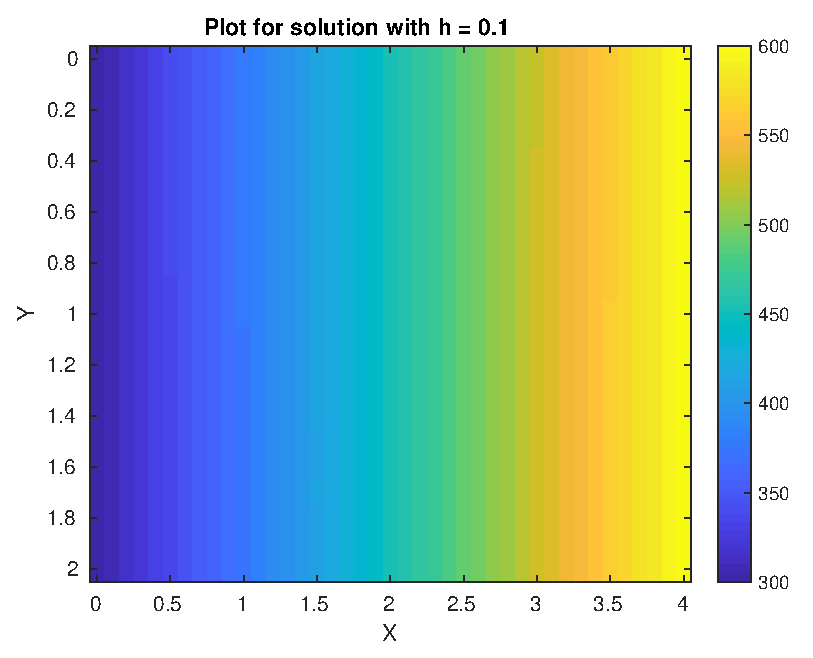
\includegraphics [width=4in]{lab4_01.eps}

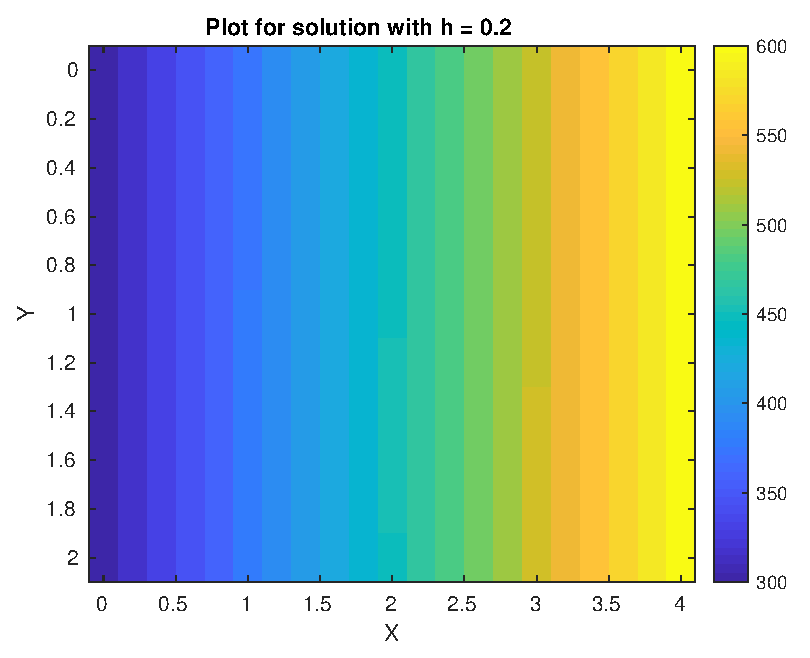
\includegraphics [width=4in]{lab4_02.eps}

\includegraphics [width=4in]{lab4_03.eps}

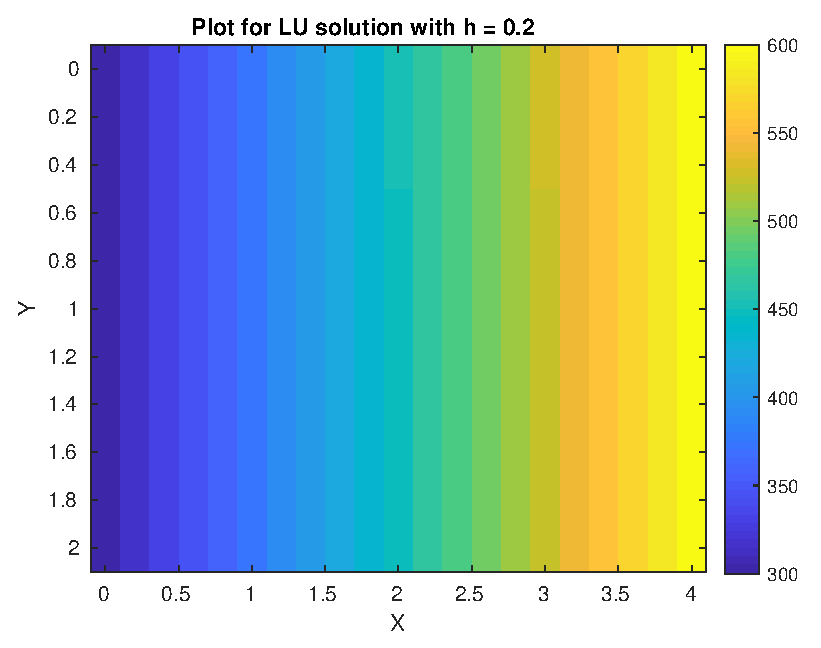
\includegraphics [width=4in]{lab4_04.eps}



\end{document}
    
